\documentclass[hyperref={pdfpagelabels=false}]{beamer}
\usepackage[utf8]{inputenc}
\usepackage[T1]{fontenc}
\usepackage{mathtools}

\usepackage{lmodern}
\usepackage{graphicx} 
\usepackage{multicol}
\usepackage{tikz}
\usepackage{framed}
\usepackage[mathscr]{euscript}
\usepackage{xcolor}
%\usepackage{cite}

\usepackage{mdframed}
\usepackage{algpseudocode}
%\usetheme{metropolis}
%\usecolortheme[named=cyan]{structure}

\definecolor{LHCblue}{RGB}{4, 114, 255}
\usecolortheme[named=LHCblue]{structure}
\usepackage[bars]{beamerthemetree}
\usetheme{Ilmenau}
\useoutertheme[subsection=true]{smoothbars}
\mdfsetup{font=\footnotesize}

\usepackage{enumerate}
\usepackage{mathrsfs}
\usepackage{amsmath,amssymb,amsthm}
\usepackage[ngerman]{babel}
\usepackage{color}


\title{Tensorstruktur der Zellmatrizen bei finiten Elementen }   
\author{Enes Witwit \\ Universität Heidelberg} 
\date{\today} 
\setbeamertemplate{navigation symbols}{}
%\usepackage{beamerthemeCambridgeUS}
\makeatother

\setbeamertemplate{headline}
{%
  \begin{beamercolorbox}[ht=3.5ex,dp=1.125ex,%
      leftskip=.3cm,rightskip=.3cm plus1fil]{section in head/foot}
    \usebeamerfont{section in head/foot}\usebeamercolor[fg]{section in head/foot}%
    \insertsectionhead
  \end{beamercolorbox}%
  \begin{beamercolorbox}[colsep=1.5pt]{middle separation line head}
  \end{beamercolorbox}
  \begin{beamercolorbox}[ht=2.5ex,dp=1.125ex,%
    leftskip=.3cm,rightskip=.3cm plus1fil]{subsection in head/foot}
    \usebeamerfont{subsection in head/foot}\insertsubsectionhead
  \end{beamercolorbox}%
  \begin{beamercolorbox}[colsep=1.5pt]{lower separation line head}
  \end{beamercolorbox}
}

\setbeamertemplate{footline}
{%
  \leavevmode%
  \hbox{\begin{beamercolorbox}[wd=.5\paperwidth,ht=2.5ex,dp=1.125ex,leftskip=.3cm,rightskip=.3cm]{author in head/foot}%
      \usebeamerfont{author in head/foot}\insertshortauthor
  \end{beamercolorbox}%
  \begin{beamercolorbox}[wd=.5\paperwidth,ht=2.5ex,dp=1.125ex,leftskip=.3cm,rightskip=.3cm plus1fil]{title in head/foot}%
    \usebeamerfont{author in head/foot}\insertshorttitle\hfill\insertpagenumber/\inserttotalframenumber
  \end{beamercolorbox}}%
  \vskip0pt%
}
\setbeamertemplate{footline}[frame number]{}

\makeatletter
\beamersetuncovermixins{\opaqueness<1>{25}}{\opaqueness<2->{15}}

\setbeamercovered{invisible}


\begin{document}
%Titlepage
\begin{frame}[noframenumbering, plain]
\titlepage
\end{frame} 


%Contents
\begin{frame}[noframenumbering, plain]
\frametitle{Inhaltsverzeichnis}
\setcounter{tocdepth}{1}
\small{ \tableofcontents}
\end{frame}

% Introduction
\section{Einleitung} 
\begin{frame}[noframenumbering, plain]
\small{\tableofcontents[currentsection]}
\end{frame}
\begin{frame}
\frametitle{Hochleistungsrechnen}
\begin{framed}
\center{\textbf{Ziel} Löse ein sehr komplexes Problem.}
\end{framed} 
\center{ \textbf{Lösungsansatz} }
Teile das komplexe Problem auf in Subprobleme (Parallelisierung).
\end{frame}


\begin{frame}
\frametitle{Initial-Problem}
\begin{framed}
\begin{equation*}
v = A(u)
\end{equation*}
A, möglicherweise nichtlinearer, finite Elemente Operator, der Vektor u als Input nimmt.
\end{framed}
Probleme 
\begin{itemize}
\item $A$ wird unter Umständen sehr groß $\rightarrow$ Speicherplatz.
\item $A$ liegt nicht mehr im Cache $\rightarrow$ Abrufen der Elemente von $A$ zeitintesiv. 
\item Berechnung des Matrix-Vektor-Produkts komplex
\end{itemize}
\end{frame}

\begin{frame}
\frametitle{Divide and Conquer}
Nach \cite{Kronbichler} können wir die Ursprungsgleichung umformen zu
\begin{equation*}
v = A(u) = \sum\limits_{k=1}^{n_{cells}} P_k^T A_k P_k u \, .
\end{equation*}
$P_k$ kümmert sich um die Einordnug der lokalen Freiheitsgrade in die globalen Freiheitsgrade.
\begin{framed}
\begin{align*}
v_k &= A_k u_k \\
A_k^{-1} v_k &= u_k
\end{align*}
\end{framed}
\end{frame}

\begin{frame}
\frametitle{Inverse/Pseudoinverse}
\begin{enumerate}
\item Tensorstruktr und Summenfaktorisierung.
\item Singulärwertzerlegung höherer Ordnung (HOSVD).
\end{enumerate}

\end{frame}


% Theorie
\section{Theorie}
\begin{frame}[noframenumbering, plain]
\small{\tableofcontents[currentsection]}
\end{frame}
\begin{frame}
\frametitle{Higher Order Singular Value Decomposition}
\begin{framed}
Defintion \\

\end{Definition}

\end{frame}

% Pseudoinverse
\section{Pseudoinverse}
\begin{frame}[noframenumbering, plain]
\small{\tableofcontents[currentsection]}
\end{frame}
\subsection{Tensorstruktur}

% Definition Masse und Laplace Matrix
\begin{frame}

\begin{framed}
\textbf{Lokale Massenmatrix}
\begin{equation*} \label{eq:mass}
M_{ik} = \int\limits_{T} \varphi_i (\bold{x}) \, \varphi_j (\bold{x}) \, d\bold{x}
\end{equation*}

\textbf{Elementsteifigkeitsmatrix der Laplace Bilinearform}
\begin{equation*}
V_{ij} = \int\limits_{T} \nabla \varphi_i(\bold{x}) \, \nabla \varphi_j(\bold{x})  d \bold{x}
\end{equation*}
\end{framed}

\begin{itemize}
\item $T$ sei die Referenzzelle für Rechtecke
\item $\varphi_i(\bold{x})$ sei eine zweidimensionale reelle Basisfunktion des diskreten Raumes $V_n$ mit $\bold{x}=(x,y)$ .
\end{itemize}

\end{frame}



% Tensorstruktur der Ansatzfunktionen
\begin{frame}
\frametitle{Tensorstruktur der Ansatzfunktionen}

\begin{equation*} \label{eq:tensor}
\varphi^{2D}_i(\bold{x})=\varphi^{2D}_{i_1+(N+1)i_2}(x,y)=\varphi^{1D}_{i_1}(x)\varphi^{1D}_{i_2}(y),
\end{equation*}

\begin{figure}[ht] 
	\centering
  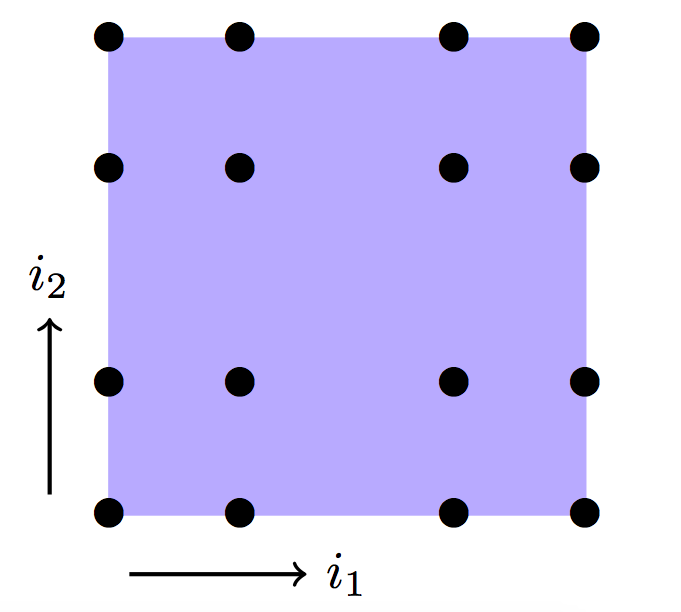
\includegraphics[width=0.3\textwidth]{lexi.png}
	\caption{ \cite[3]{Teachlet}}
	\label{fig:lexi}
\end{figure}

\end{frame}

\begin{frame}
\frametitle{Tensorstruktur der Massenmatrix}
Es seien $\bold{x}_q=(x_{q1},x_{q2})$ die Stützstellen und $\bold{w}_q=w_{q1}w_{q2}$ die Gewichte der Gauss Quadratur.
\begin{equation*} \label{eq:massapprox}
\begin{aligned}
M_{ij} &= \int\limits_{T} \varphi_i (\bold{x}) \, \varphi_j (\bold{x}) \, d\bold{x} \\ \pause
&\approx  \sum\limits_{q=1}^Q \bold{w}_q \, \, \varphi_i (\bold{x}_q) \, \varphi_j (\bold{x}_q) \\ \pause
&= \sum\limits_{q_1=1}^{Q_{1D}} \sum\limits_{q_2=1}^{Q_{1D}} \varphi_{i_1}(x_{q1}) \varphi_{i_2}(x_{q2}) \varphi_{j_1}(x_{q1}) \varphi_{j_2}(x_{q2}) \, w_{q1} w_{q2} \\ 
&= \sum\limits_{q_1=1}^{Q_{1D}} w_{q1} \varphi_{i_1}(x_{q1}) \varphi_{j_1}(x_{q1}) \sum\limits_{q_2=1}^{Q_{1D}} w_{q2} \varphi_{i_2}(x_{q2}) \varphi_{j_2}(x_{q2}) \, . 
\end{aligned}
\end{equation*}
\end{frame}

\begin{frame}
\textbf{Definiere} \\
\begin{itemize}
\item Es sei $\mathcal{N}$ eine Matrix mit $\mathcal{N}_{iq}=\varphi_i(\bold{x}_q)$.
\item Es sei $\mathcal{W}$ eine Matrix mit $\mathcal{W}_{ii}=\bold{w}_i$, sonst Nullen.
\end{itemize}
Dann können wir die Massenmatrix schreiben als
\begin{equation*}
M = \underbrace{\mathcal{N} \mathcal{W}}_{:=\mathcal{W}_N} \mathcal{N}^T. = \mathcal{W}_N \mathcal{N}^T
\end{equation*}
\pause
\textbf{Nutze Tensorstruktur der Ansatzfunktionen}
\begin{equation*}
\begin{aligned}
\mathcal{N} &= \mathcal{N}^{1D} \otimes \mathcal{N}^{1D} \\
\mathcal{W}_N &= \mathcal{W}_N^{1D} \otimes \mathcal{W}_N^{1D}
\end{aligned}
\end{equation*}
\end{frame}

\begin{frame}
\frametitle{Tensorstruktur der Massenmatrix}
\begin{framed}
\begin{equation*}
\begin{aligned}
M &= \mathcal{W}_N \mathcal{N}^T \\
&= (\mathcal{W}_N^{1D} \otimes \mathcal{W}_N^{1D})(\mathcal{N}^{1D} \otimes \mathcal{N}^{1D})^T \\
&= (\mathcal{W}_N^{1D} \otimes \mathcal{W}_N^{1D})((\mathcal{N}^{1D})^T \otimes (\mathcal{N}^{1D})^T) \\
&= (\mathcal{W}_N^{1D} (\mathcal{N}^{1D})^T) \otimes  (\mathcal{W}_N^{1D} (\mathcal{N}^{1D})^T) 
\end{aligned}
\end{equation*}
\end{framed}
\end{frame}

\begin{frame}
\frametitle{Pseudoinverse der Massenmatrix}
\begin{equation*}
\begin{aligned}
M^+ & = [(\mathcal{W}_N^{1D} (\mathcal{N}^{1D})^T) \otimes  (\mathcal{W}_N^{1D} (\mathcal{N}^{1D})^T)]^+ \\ &= (\mathcal{W}_N^{1D} (\mathcal{N}^{1D})^T)^+ \otimes  (\mathcal{W}_N^{1D} (\mathcal{N}^{1D})^T)^+ 
\end{aligned}
\end{equation*}
\end{frame}





\begin{frame}
\frametitle{Tensorstruktur der Laplace Bilinearform}
\begin{equation*}
\begin{aligned}
V_{ij} &= \int\limits_{T} \nabla \varphi_i(\bold{x}) \, \nabla \varphi_j(\bold{x})  d \bold{x} \\ 
&= \int\limits_{T}( \partial_{x_1}  \varphi_i(\bold{x})  \partial_{x_1} \varphi_j(\bold{x})) + ( \partial_{x_2} \varphi_i(\bold{x})  \partial_{x_2} \varphi_j(\bold{x})) \, d\bold{x} \\
&= \int\limits_{T}( \partial_{x_1}  \varphi_i(\bold{x})  \partial_{x_1} \varphi_j(\bold{x})) + ( \partial_{x_2} \varphi_i(\bold{x})  \partial_{x_2} \varphi_j(\bold{x})) \, d\bold{x} \\ &= \int\limits_{T} \partial_{x_1}  \varphi_i(\bold{x})  \partial_{x_1} \varphi_j(\bold{x}) d\bold{x} + \int\limits_{T}  \partial_{x_2} \varphi_i(\bold{x})  \partial_{x_2} \varphi_j(\bold{x}) \, d\bold{x} \\
&= \underbrace{\sum\limits_{q=1}^{(N+1)^2} \bold{w}_q \partial_{x_1}  \varphi_i(\bold{x}_q)  \partial_{x_1} \varphi_j (\bold{x}_q)}_{K^1} + \underbrace{\sum\limits_{q=1}^{(N+1)^2} \bold{w}_q  \partial_{x_2} \varphi_i(\bold{x}_q)  \partial_{x_2} \varphi_j(\bold{x}_q)}_{K^2} \, 
\end{aligned}
\end{equation*}
\end{frame}

\begin{frame}
\begin{equation*}
\begin{aligned}
K_{ij}^1 &=\sum\limits_{q=1}^{(N+1)^2} \bold{w}_q \partial_{x_1}  \varphi_i(\bold{x}_q)  \partial_{x_1} \varphi_j (\bold{x}_q) \\ &= \sum\limits_{q_1=1}^{N} \sum\limits_{q_2=1}^{N} w_{q1}w_{q2} \partial_{x_1}  \varphi_{i1}(x_{q1})\varphi_{i2}(x_{q2})  \partial_{x_1} \varphi_{j1} (x_{q1})\varphi_{j2} (x_{q2}) \\
&=  \sum\limits_{q_1=1}^{N} \sum\limits_{q_2=1}^{N} w_{q1}w_{q2} \varphi'_{i1}(x_{q1})\varphi_{i2}(x_{q2})  \varphi'_{j1} (x_{q1})\varphi_{j2} (x_{q2}) \\ 
&= \sum\limits_{q_1=1}^{N} w_{q1} \varphi'_{i1}(x_{q1}) \varphi'_{j1} (x_{q1}) \sum\limits_{q_2=1}^{N} w_{q2} \varphi_{i2}(x_{q2})  \varphi_{j2} (x_{q2}) 
\end{aligned}
\end{equation*}
\end{frame}

\begin{frame}
\textbf{Definiere}
\begin{itemize}
\item Es sei $\widehat{\mathcal{N}}^{1D}$ eine Matrix mit $\widehat{\mathcal{N}}^{1D}_{ik}=\varphi'^{1D}_i(x_k)$
\item Dementsprechend ist $\widehat{\mathcal{W}}^{1D}_N$ eine Matrix, die aufgebaut ist wie $\mathcal{W}^{1D}_N$, mit dem Unterschied, dass sie die Evaluationen der ersten Ableitungen der Ansatzfunktionen beinhaltet.
\end{itemize}
\pause
\textbf{Dann} können wir $K_1,K_2$ schreiben als
\begin{align*}
K_1 &= (\widehat{\mathcal{W}}_N^{1D} (\widehat{\mathcal{N}}^{1D})^T) \otimes (\mathcal{W}_N^{1D}(\mathcal{N}^{1D})^T) \\
K_2 &= (\mathcal{W}_N^{1D} (\mathcal{N}^{1D})^T) \otimes (\widehat{\mathcal{W}}_N^{1D} (\widehat{\mathcal{N}}^{1D})^T)
\end{align*}
\begin{framed}
\begin{equation*}
V =\widehat{\mathcal{W}}_N \widehat{\mathcal{N}}^T \otimes \mathcal{W}_N \mathcal{N}^{T} + \mathcal{W}_N \mathcal{N}^{T}\otimes \widehat{\mathcal{W}}_N \widehat{\mathcal{N}}^T.
\end{equation*}
\end{framed}
\end{frame}

\begin{frame}
\frametitle{Problem bei Laplace}
\textbf{Problem } Die Addition in der Tensorstruktur macht unseren ersten Ansatz hinfällig. \\
\textbf{Idee } Vereinfache die Form durch geeignete Basiswahl und dann sehen wir weiter. Wir wählen geeignete Basis, sodass $ \, \mathcal{W}_N \mathcal{N}^{T} = I_n \, $.

Folgende Basispolynome bieten sich an:
\begin{framed}
\begin{equation*}
\varphi^{1D}_i (x_k) = \dfrac{1}{ \sqrt{w_i} } l_i (x_k) = 
\begin{cases}
\dfrac{1}{ \sqrt{w_i} } \, \text{ , wenn } i=k  \\
0  \, \, \, \, \, \, \, \, \, \, \, \text{ , sonst. }
\end{cases}
\end{equation*}
Die Funktion $l_i(x_k)$ bezeichnet das $i-te$ Lagrange Polynom.
\end{framed}
\end{frame}


% Effiziente Berechnung
\section{Effiziente Berechnung}
\begin{frame}[noframenumbering, plain]
\small{\tableofcontents[currentsection]}
\end{frame}
In Kapitel 3 haben wir uns zwei Möglichkeiten angeschaut, das Matrix-Vektor Produt zu berechnen mit der Pseudoinversen. Beide Alternativen bargen eine Tensorprodukt Struktur, in Form des Matrix-Kronecker Produkt.

Das heißt um dies effizient zu implementieren sollten wir uns Gedanken dadrüber machen wie wir diese Struktur ausnutzen können.

Im Exa-dg-teachlet wird eine Strategie vorgestellt ein Matrix-vektor Produkt mit Kronecker Matrizen also $z=(\mathcal{B} \otimes \mathcal{A})y$ berechnet werden kann.

Sei $\mathcal{A} \in \mathbb{R}^{m \times n}$ und $\mathcal{B} \in \mathbb{R}^{p \times q}$. Das Kronecker Produkt dieser Matrizen kann man schreiben als, 
\begin{equation*}
\mathcal{B} \times \mathcal{A} =
\begin{pmatrix}
b_{11}\mathcal{A} & \dots  & b_{1q}\mathcal{A} \\
\vdots & \ddots & \vdots \\
b_{p1}\mathcal{A} & \dots & b_{pq}\mathcal{A} \\
\end{pmatrix}
\end{equation*}

Nun wir sehen also die sich wiederholende Struktur von $\mathcal{A}$. Genau diese wollen wir uns nun zu nutze machen. Nehmen wir an y sei geordnet in der Indexierung.
\begin{equation*}
y = (y_1,y_2,\dots,y_n,\dots,\dots,y_{(q-1)n+1},y_{(q-1)n+2},\dots,y_{qn})^T
\end{equation*}

Wir denken uns nun die Faktoren $b_{ij}$ die mit $\mathcal{A}$ multipliziert werden erstmal weg. Definiere $y^{(1)}=(y_1,y_2,\dots,y_n)^T$.

\begin{equation*}
w^{(1)}=
\begin{pmatrix}
w_1 \\ \vdots \\ w_m 
\end{pmatrix}
=
\begin{pmatrix}
a_{11} & \dots & a_{1n} \\
\vdots & \dots & \vdots \\
a_{m1} & \dots & a_{mn} \\
\end{pmatrix}
\begin{pmatrix}
y_1 \\ \vdots \\ y_n
\end{pmatrix}
= \mathcal{A}y^{(1)}
\end{equation*}

Auf ähnliche Weise können wir uns $y^{(2)}=(y_{n+1},\dots,y_{2n})^{T}$ definieren und dann
\begin{equation*}
w^{(2)} = \mathcal{A}y^{(2)}
\end{equation*}

Wir führen dies so weiter und erhalten

\begin{equation*}
w=( (w^{(1)})^T , \dots, (w^{(q)})^T) \in \mathbb{R}^{mq}
\end{equation*}

Nun müssen wir die Informationen der Matrix B noch mit reinbringen.
%%%%%%%%%%%%%%%%%%%

Nun haben wir uns mit Hilfe der Tucker Dekomposition eine Herleitung für die Pseudoinverse erarbeitet. Nun geht es um die effiziente Berechnung dieser Formel. Dazu wollen wir uns die Summenfaktorisierung zu nutze machen, wie sie auch in \cite[9-11]{Teachlet} vorgeschlagen wird.
Sei $\mathcal{A} \in \mathbb{R}^{I_{1} \times \dots \times I_{n}}$ .
Die Formel für die Pseudoinverse lautet:

\begin{equation} \label{eq:pinv}
\mathcal{A}^{\dagger} = \mathcal{S}^{\dagger} \times_{n=1}^{N} U^{ (n) ^{T} }
\end{equation}

Wobei $\mathcal{S} \in \mathbb{R}^{I_{1} \times \dots \times I_{n}}$ und $U^{(n)} \in \mathbb{R}^{J_{n} \times I_{n}}$
Man kann \ref{eq:pinv} nach \cite[462]{Kolda} äquivalent umformen zu

\begin{equation}
\begin{aligned}
\mathcal{A}^{\dagger}_{(n)}  &= U^{ (n) ^{T} }  \mathcal{S}^{\dagger}_{(n)} ( U^{ (N) ^{T} } \otimes \dots \otimes U^{ (n+1) ^{T} } \otimes U^{ (n-1) ^{T} } \otimes \dots \otimes U^{ (1) ^{T} })^{T} \\ \iff
\mathcal{A}^{\dagger}_{(n)} &= U^{ (n) ^{T} }  \mathcal{S}^{\dagger}_{(n)} ( U^{ (N)  } \otimes \dots \otimes U^{ (n+1) } \otimes U^{ (n-1) } \otimes \dots \otimes U^{ (1) })
\end{aligned}
\end{equation}

Nun betrachten wir uns das Matrix-Vektor Produkt und überlegen uns wie wir uns die Strukturen dort zu nutze machen.

\begin{equation} \label{eq:pinvv}
\begin{aligned}
\mathcal{A}^{\dagger}_{(n)}v&= U^{ (n) ^{T} }  \mathcal{S}^{\dagger}_{(n)} ( U^{ (N)  } \otimes \dots \otimes U^{ (n+1) } \otimes U^{ (n-1) } \otimes \dots \otimes U^{ (1) }) v
\end{aligned}
\end{equation}

Wir schauen uns die Struktur mal für den Fall, dass $\mathcal{A} \in \mathbb{R}^{I_{1} \times \dots \times I_{4}}$. Das heißt \ref{eq:pinvv} reduziert sich auf:

\begin{equation} \label{eq:pinvcase}
\begin{aligned}
\mathcal{A}^{\dagger}_{(n)}v&= U^{ (n) ^{T} }  \mathcal{S}^{\dagger}_{(n)} ( U^{ (N_{1})  } \otimes U^{ (N_{2})}  \otimes U^{ (N_{3}) }) v
\end{aligned}
\end{equation}
mit $N_{i} \neq n$.

Zu Zwecken der Veranschaulichung nehmen wir eine Umdefinierung vor:
$A := U^{(N_3)}, B:= U^{(N_2)}, C:=U^{(N_1)}$.
Wenn wir uns die Struktur in der Klammer anschauen sieht diese wie folgt aus

\begin{equation} z:=
\begin{pmatrix}
c_{11} b_{11} A & \dots  & c_{11} b_{1n} A & \dots & \dots & c_{1n}b_{11}A & \dots & c_{1n}b_{1n}A  \\

\vdots & \vdots & \ddots & \ddots  & \ddots & \vdots & \vdots & \vdots \\
c_{11} b_{n1} A & \dots  & c_{11} b_{nn} A & \dots & \dots & c_{1n}b_{n1}A & \dots & c_{1n}b_{nn}A  \\
c_{21} b_{n1} A & \dots  & c_{21} b_{nn} A & \dots & \dots & c_{2n}b_{n1}A & \dots & c_{2n}b_{nn}A  \\
\vdots & \vdots & \ddots & \ddots  & \ddots & \vdots & \vdots & \vdots \\
c_{n1} b_{n1} A & \dots  & c_{n1} b_{nn} A & \dots & \dots & c_{nn}b_{n1}A & \dots & c_{nn}b_{nn}A  \\
\end{pmatrix} * v
\end{equation}

Wir sehen hier sich zwei wiederholende Strukturen die wir ausnutzen können um bei einem Matrix-Vektor Produkt operationen zu sparen.

\begin{equation} \label{eq:matrix} z=
\begin{pmatrix}
c_{11} \textcolor{green}{b_{11}} \textcolor{red}{A} & \dots  & c_{11} \textcolor{green}{b_{1n}} \textcolor{red}{A} & \dots & \dots & c_{1n}\textcolor{green}{b_{11}}\textcolor{red}{A} & \dots & c_{1n}\textcolor{green}{b_{1n}}\textcolor{red}{A}  \\

\vdots & \vdots & \ddots & \ddots  & \ddots & \vdots & \vdots & \vdots \\
c_{11} \textcolor{green}{b_{n1}} \textcolor{red}{A} & \dots  & c_{11} \textcolor{green}{b_{nn}} \textcolor{red}{A} & \dots & \dots & c_{1n}\textcolor{green}{b_{n1}}\textcolor{red}{A} & \dots & c_{1n}\textcolor{green}{b_{nn}}\textcolor{red}{A}  \\
c_{21} \textcolor{green}{b_{n1}} \textcolor{red}{A} & \dots  & c_{21} \textcolor{green}{b_{nn}} \textcolor{red}{A} & \dots & \dots & c_{2n}\textcolor{green}{b_{n1}}\textcolor{red}{A} & \dots & c_{2n}\textcolor{green}{b_{nn}}\textcolor{red}{A}  \\
\vdots & \vdots & \ddots & \ddots  & \ddots & \vdots & \vdots & \vdots \\
c_{n1} \textcolor{green}{b_{n1}} \textcolor{red}{A} & \dots  & c_{n1} \textcolor{green}{b_{nn}} \textcolor{red}{A} & \dots & \dots & c_{nn}\textcolor{green}{b_{n1}}\textcolor{red}{A} & \dots & c_{nn}\textcolor{green}{b_{nn}}\textcolor{red}{A}  \\
\end{pmatrix} * v
\end{equation}

Nun wollen wir uns dies zu nutze machen. Wir schauen uns erstmal die einzelnen Einträge von z an und bekommen. Vorher definieren wir unser v um zu einem Tensor $\mathcal{V} \in \mathbb{R}^{I_1 \times I_2 \times I_3} $. Der erste Index repräsentiert in welcher Spalteneintrag von C wir uns befinden, der zweite in welchem Spalteneintrag von B und der Dritte in welchem Spalteneintrag von A. 
\begin{equation} \label{eq:zold}
\begin{aligned}
z_{1} = \mathcal{V}(1,1,1) c_{11} \textcolor{green}{b_{11}} \textcolor{red}{a_{11}}+ \dots +  \mathcal{V}(1,1,n) c_{11} \textcolor{green}{b_{11}} \textcolor{red}{a_{1n}} + \dots  +  \mathcal{V}(1,n,1)c_{11} 
\textcolor{green}{b_{1n}} \textcolor{red}{a_{11}} \\ + \dots +  \mathcal{V}(n,1,1) c_{1n} \textcolor{green}{b_{11}} \textcolor{red}{a_{11}} + \dots +  \mathcal{V}(n,n,n) c_{1n} \textcolor{green}{b_{1n}} \textcolor{red}{a_{1n}}
\end{aligned}
\end{equation}
Definiere $w_{\textcolor{red}{1}}(i,j) :=\mathcal{V}(i,j,1) a_{\textcolor{red}{1}1}+\dots+\mathcal{V}(i,j,n) a_{\textcolor{red}{1}n}$. Dann erhalten wir:
\begin{equation*}
\begin{aligned}
z_{1}= w_1(1,1) c_{11} b_{11} + \dots +   w_1(1,n) c_{11} b_{1n} + \dots + w_1(n,1) c_{1n} b_{11}  + \dots +  w_1(n,n) c_{1n} b_{1n} 
\end{aligned}
\end{equation*}

Damit haben wir uns die sich wiederholende Struktur von der Matrix \textcolor{red}{A} zu nutze gemacht. Im nächsten Schritt machen wir uns die sich wiederholende Struktur von $\textcolor{green}{b_{ij}}$ zu nutze.
Definiere hierfür $\textswab{W}_{\textcolor{red}{1},k} (i):= w_k(i,1) b_{\textcolor{red}{1}1} + \dots + w_k(i,n) b_{\textcolor{red}{1}n}$. Damit erhalten wir:

\begin{equation} \label{eq:znew}
\begin{aligned}
z_{1}= \textswab{W}_{1,1}(1) c_{11}  + \dots +  \textswab{W}_{1,1}(n) c_{1n} 
\end{aligned}
\end{equation}

Wir wollen nun $z$ genau so umformen wie wir das auch für v gemacht haben. Damit erhalten wir für allgemeines $z_{i}$ folgende Formel:
\begin{equation}
\mathcal{Z}(i,j,k) = \textswab{W}_{j,k}(1) c_{i1}  + \dots +  \textswab{W}_{j,k}(n) c_{in} 
\end{equation}
Wobei j und k den Zeilen jeweils in den Matrizen B und C entsprechen. 

Der komplette Algorithmus würde nun wie folgt aussehen:
\begin{algorithmic}
\For {k=1 < n }
	\For {i= 1 < n }
		\For {j= 1 < n }
			\State $w_{k}(i,j) = \mathcal{V}(i,j,1)a_{k1} + \dots + \mathcal{V}(i,j,n)a_{kn}$
		\EndFor
	\EndFor
\EndFor
\For {k=1 < n }
	\For {i= 1 < n }
		\For {j= 1 < n }
			\State $\textswab{W}_{i,j} (k):= w_k(i,1) b_{11} + \dots + w_k(i,n) b_{1n}$
		\EndFor
	\EndFor
\EndFor
\For {k=1 < n }
	\For {i= 1 < n }
		\For {j= 1 < n }
			\State $\mathcal{Z}(i,j,k) = \textswab{W}_{j,k}(1) c_{i1}  + \dots +  \textswab{W}_{j,k}(n) c_{in}$ 
		\EndFor
	\EndFor
\EndFor
\end{algorithmic}

 
Wenn wir annehmen, dass die Matrizen $A,B,C \in \mathbb{R}^{n \times n}$. Dann haben wir bei \ref{eq:matrix} eine Matrix-Vektor Multiplikation von einer Matrix der Größe $n^{3} \times n^{3}$. Dementsprechend hätten wir $n^{6}$ Multiplikationen und $n^{6}$ Additionen. Die Komplexität des vorgeschlagenen Algorithmuses reduziert sich auf $3n^{4}$ Multiplikationen und genau so viele Additionen.
Ein enorme Reduktion, vor allem für großes n.

% Effiziente Berechnung
\section{Resultate}
\begin{frame}[noframenumbering, plain]
\small{\tableofcontents[currentsection]}
\end{frame}
\begin{frame}
\frametitle{Resultate}
Wir haben zwei Möglichkeiten betrachtet die Pseudoinverse der zu untersuchunden Bilinearformen herzuleiten
\begin{enumerate}
\item Ausnutzung der Tensorstruktur und Herleitung einer einfachen Form
\item Universellen Ansatz über die HOSVD
\end{enumerate}
Die beiden Methoden haben ihre Vor und Nachteile. Die erste Methode:
\begin{itemize}
\item nicht flexibel
\item individueller Lösungsansatz für jede Bilinearform
\item Komplexitätsklasse $O(N^3)$
\end{itemize}
Die zweite Methode über die HOSVD:
\begin{itemize}
\item flexibilität
\item Komplexitätsklasse vom $O(N^6)$
\end{itemize}
\end{frame}
\begin{frame}
\frametitle{Zukunft}
In Zukunft kann man 
\begin{itemize}
\item Mehr Bilinearformen auf Tensorstrukturen untersuchen
\item Das Kommunikationsverhalten des $n-mode$ Produkt  mit anderen Operatoren näher betrachten
\item Effizientere Matrix-Matrix Multiplikation
\item Unsere definierte Entfaltung bezüglich der HOSVD untersuchen
\begin{equation*}
\mathcal{X}^{(p)} v = [(U^{(1)} \otimes U^{(2)}) \mathcal{G}^{(p)} (U^{(3)} \otimes U^{(4)})] v
\end{equation*}
\end{itemize}
\end{frame}
\begin{frame}
\frametitle{Framework für Testzwecke und Inspiration}
https://github.com/Oldbridgegeek/pcvt
\end{frame}

\section*{Literatur}
\begin{frame}
\bibliographystyle{alpha}
\bibliography{literatur}
\end{frame}



\end{document}